\chapter{Models and Experiments}
\label{sec:experiment}
\section{Context Size}
\cite{Mikolov:13a} describe in their work how context size affects the type and quality of word vectors. One of the observations is that a smaller context size tend to capture syntactic similarity to a much better extent. As we increase the context size, vectors tend to capture more of semantic similarity.
\begin{figure}[]
	\centering
	\begin{subfigure}{\linewidth}
	\includegraphics[scale=0.08]{tsne_5.ps}
	\caption{}
	\label{fig:5K_hindi_zoom1}
	\end{subfigure}
	\newline
	\begin{subfigure}{\linewidth}
	\includegraphics[scale=0.08]{tsne_10.ps}
	\caption{}
	\end{subfigure}
	\newline
	\caption{High Dimensional representation of Wiki Text with a) Context Size 5 b) Context Size 10}
	\label{fig:tsne_5_10}
\end{figure}

Figure \ref{fig:tsne_5_10} shows how the high dimensional representation changes when we change the context size. The embeddings were formed with context sizes 5 and 10 by training on Latest Wikipedia dump. We see that 5.1(a), has words \emph{\{high,higher,highest\}} very close to each other which is in accordamce to our argument that smaller context size promotes syntactical similarity whereas these words are farther when we increase the context size. From 5.1(b), we can see that there is a larger semantic difference between two clusters of words:\emph{\{wikiproject,wikipeda\}} and \emph{\{facebook,html,id\}}. This again justifies our argument that larger context size favors more of semantic similarity than syntactic similarity.

\begin{figure}[ht!]
\centering
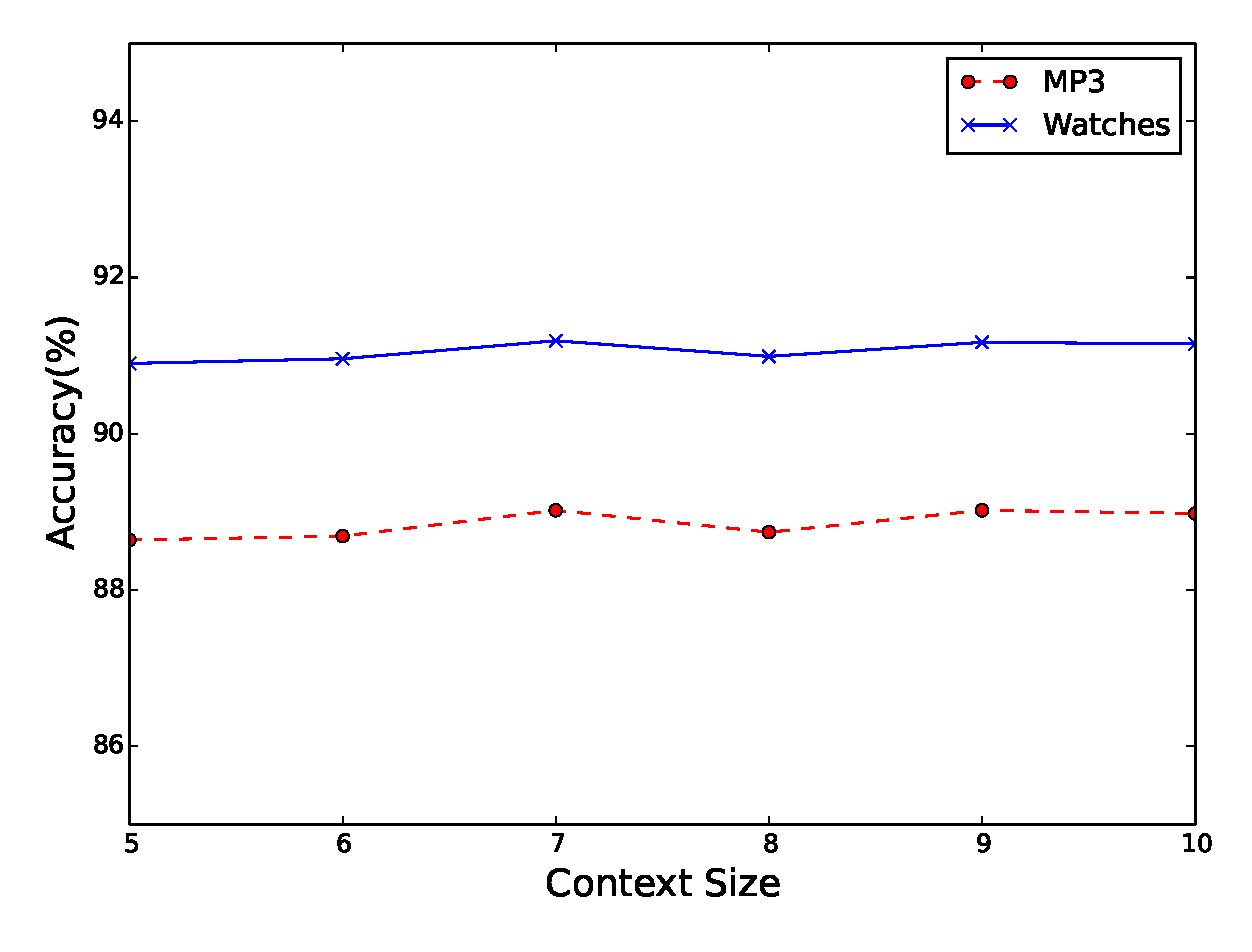
\includegraphics[width=140mm, height=110mm]{context_size.eps}
\caption{Variation of Accuracy with Different Context Size on Watches and MP3 Datasets. \label{fig:context_size}}
\end{figure}
We try to look how context size affects the accuracy on two amazon datasets, Watches and MP3.
Figure 5.2 depicts the accuracies obtained by varying the context size from 5 to 10. In both the cases, we find a peak at context size 7. There is an increase from 5 to 7 which denotes increase of context strength. As a result, we see increase in accuracies. Once the context size goes beyond a threshold, the semantic counterpart dominates which attains maximum at context size 10.\\
We also see that larger data size or training data affects the accuracy on test set. In this case, \emph{Watches} dataset is larger than \emph{MP3} dataset.\\


\section{SkipGram or CBOW}
SkipGram model tends to predict a context given a word whereas CBOW model predicts a word given a context. It seems intuitive and also from observation~\cite{Mikolov:13b} that SkipGram will perform better on semantic tasks and CBOW on syntactic tasks. We now try to evaluate how they differ on classification accuracies on the two datasets: \emph{Watches} and \emph{MP3}.
\begin{figure}[ht!]
\centering
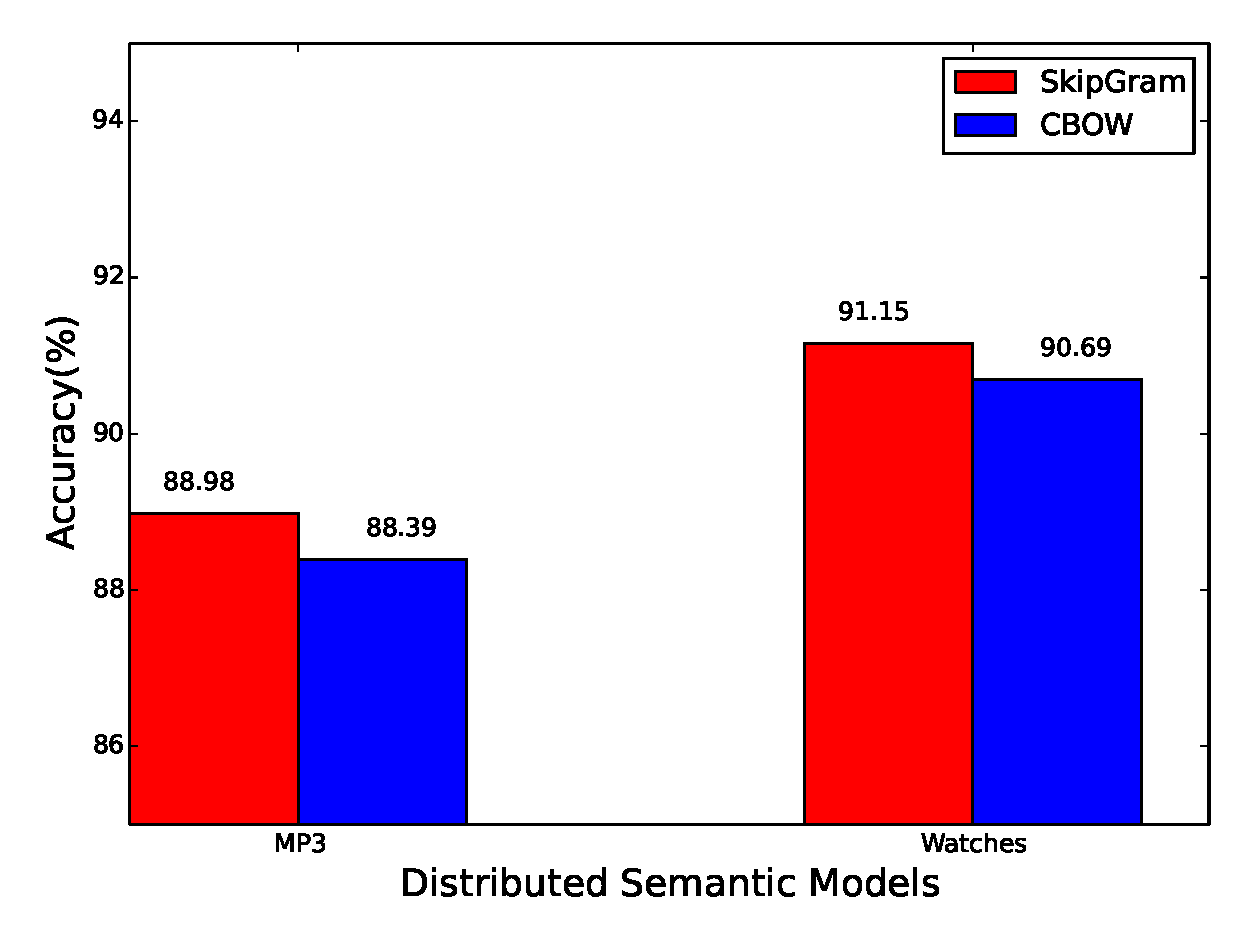
\includegraphics[width=140mm, height=110mm]{accuracy_sgcbow.eps}
\caption{Variation of Accuracy with Different Context Size on Watches and MP3 Datasets. \label{fig:accuracy_sgcbow}}
\end{figure}
Figure \ref{fig:accuracy_sgcbow} show that skipgram outperforms CBOW on sentiment classification task. It can be justified by the fact that sentiment inclination of a document is more oriented towards semantics of that document rather than just syntax and our results clearly demonstrate this fact.

A workflow defined as a graphic summary of the following has been depicted in Figure \ref{work_flow}.
We also trained our skip-gram model on Hindi Wikipedia text dump (approx. 290MB) containing around 24M words with 724K words in the vocabulary. This provided us with good embeddings due to larger size and contents from almost all domains.

The quality of word vectors can be evaluated by comparing them with words which are closer to them semantically and syntactically. This is usually done via cosine similarity.  Another evaluation can be done through tSNE~\cite{Maaten:08} which helps in visualization which maps each high-dimensional data point to a two or three-dimensional map. In our experiment, we took 5K words and plotted
them with tSNE (fig.~\ref{fig:5K_hindi_zoom}). 

\begin{figure}[ht!]
\centering
\includegraphics[width=140mm, height=110mm]{tsne.ps}
\caption{Variation of Accuracy with Different Context Size on Watches and MP3 Datasets. \label{fig:context_size}}
\end{figure}

%\begin{figure}[ht!]
%\centering
%\includepdf[width=80mm]{tsne.pdf}
%\includegraphics[width=80mm]{tsne.pdf}
%\caption{t-SNE visualization of the top 5000 Hindi Words in high dimensional space.  (Magnify to see details).}
%\label{fig:5K_hindi_zoom}
%\end{figure}

Figure \ref{fig:5K_hindi_zoom} gives a closer look into few clusters which depicts the relation between words in high dimensional space. Figure \ref{fig:5K_hindi_zoom1} shows that words such as 
%{\dn mO\8{j}d} and {\dn uplND} 
are closer to each other but farther from words such as 
%{\dn \31EwyAdA} and {\dn aEDk}.

\begin{figure}[ht!]
    \centering
    \begin{subfigure}{.4\linewidth}
        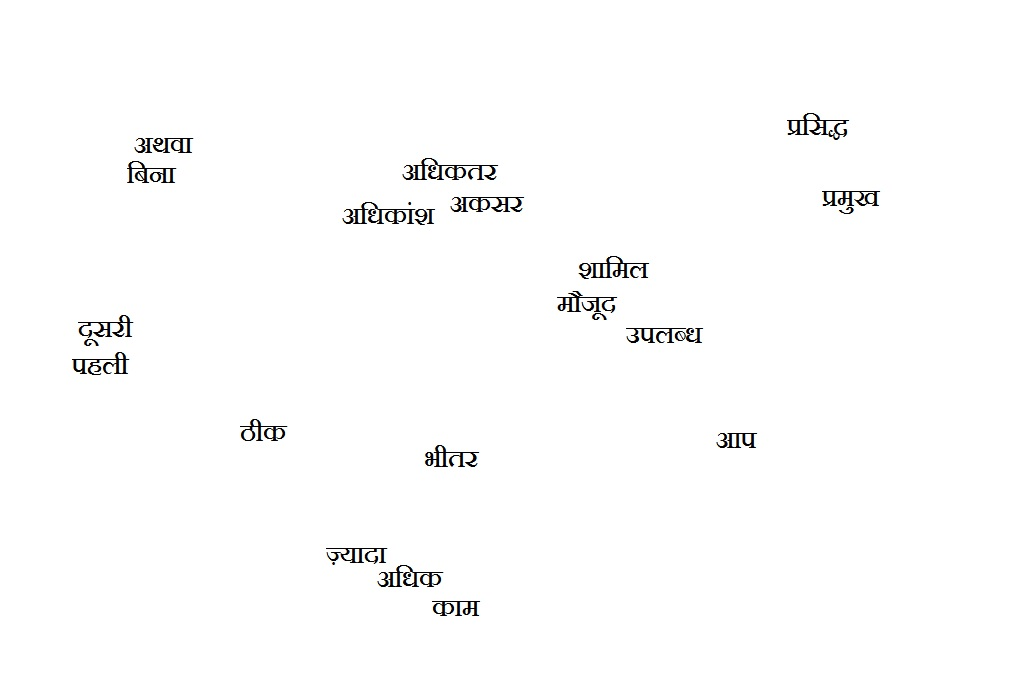
\includegraphics[scale=0.5]{5K_hindi_zoom1.eps}
        \caption{}
        \label{fig:5K_hindi_zoom1}
    \end{subfigure}
    \newline
    \begin{subfigure}{.4\linewidth}
        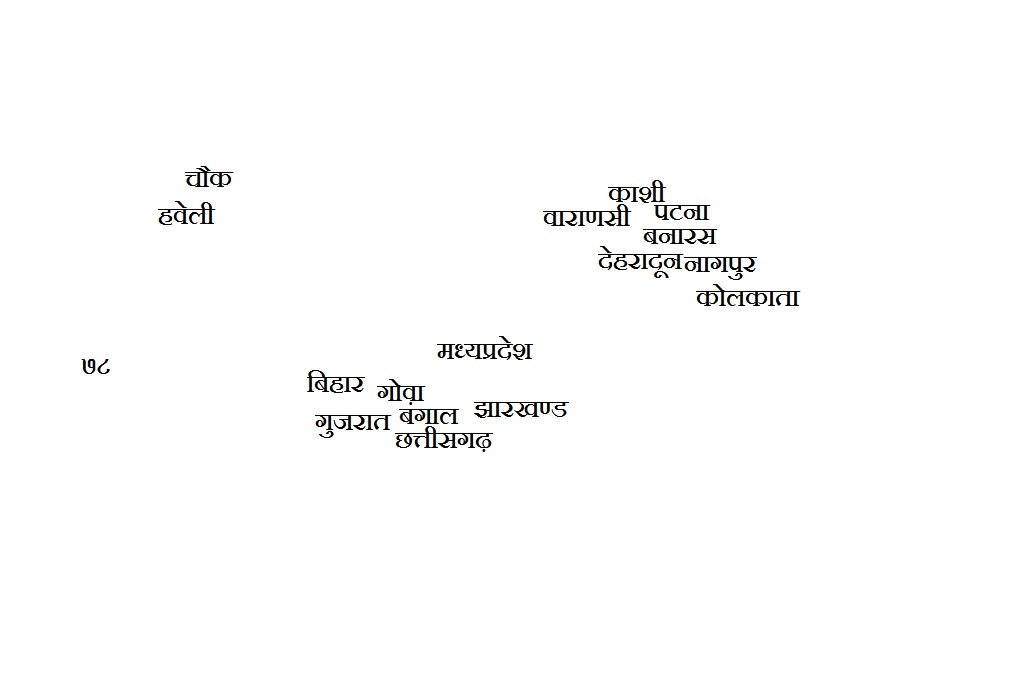
\includegraphics[scale=0.5]{5K_hindi_zoom2.eps}
        \caption{}
    \end{subfigure}
    \newline
    \begin{subfigure}{.4\linewidth}
        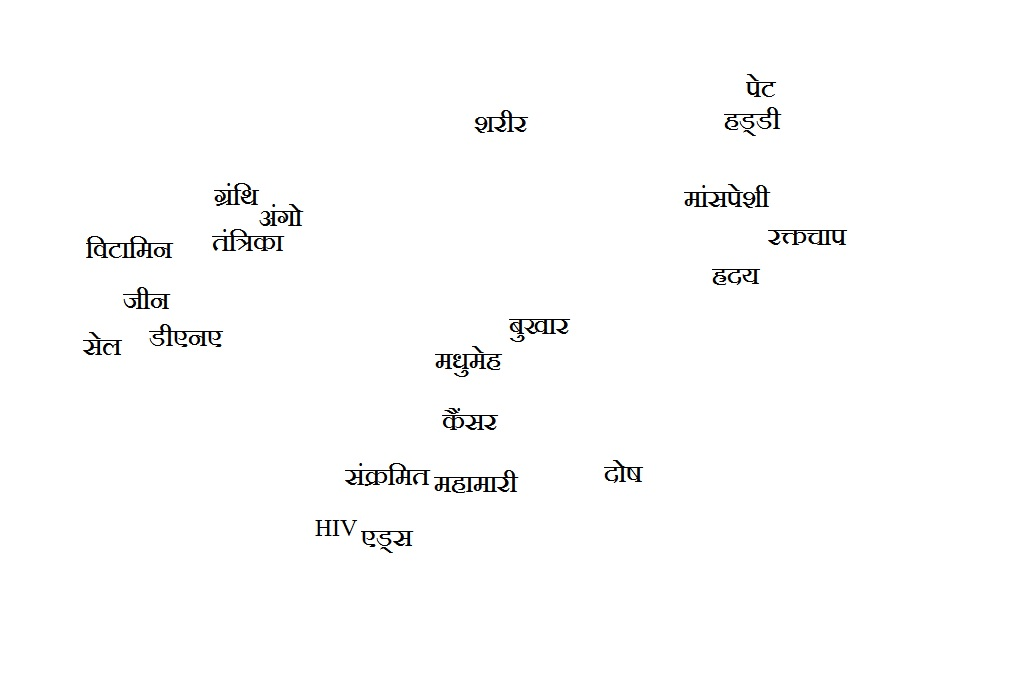
\includegraphics[scale=0.5]{5K_hindi_zoom3.eps}
        \caption{}
    \end{subfigure}
    \caption{A closer look at two clusters in the visualization showing a) quantity relations, b) locations and c) diseases.}
    \label{fig:5K_hindi_zoom}
\end{figure}

\section{Skip-Gram and \emph{tf-idf} based Word Vectors}
In this experiment, we first generated 300-dimensional word vectors by training skip-gram model on both review corpus. The context size was taken as 5. We then averaged-out word vectors for each document to create document vectors. This now acts as a feature set for that particular document.
We also created \emph{tf-idf} vectors for each document. This can be seen as a vector representation of that particular document. We then concatenated these document vectors with document vectors obtained after averaging-out word vector of each document. In this case, the dimension of each word vector obtained from skip-gram training was 500.

\section{Skip-Gram and \emph{tf-idf} based Word Vectors without stop-words}
In this experiment, we filtered out stop-words on the basis of their frequency in the corpus. Words which had very high or very low frequency were pruned as they had negligible contribution to the sentiment polarity of a document. This is a noise-reduction step and gives better results.

\section{Weighted Average Word Vectors}
Algorithm \ref{alg:weighted_average} presents a new approach to build document vectors using distributional semantics. Refer to \ref{sec:hindi_results} to see how this new technique has improved sentiment classification on Hindi reviews.
\RestyleAlgo{boxruled}
\LinesNumbered
\begin{algorithm}[ht!]
\large
\textbf{Skip-Gram}: Train skip-gram model on text to obtain word vectors.\\
\textbf{idf Calculation}: Calculate \emph{idf} value of each word with respect to given document (Refer \ref{subsec:tfidf}).\\
\textbf{Additive Composition}: For each document, $\sum_{i}(idf_i \times WordVector_i)$ is the document vector.\\
\textbf{Feature Set}: Repeat 3 for each document in training and test set to build document vectors.\\
\textbf{Classification}: Use a binary classification algorithm(SVM or Logistic Regression) to classify each test sample as positive or negative.
\caption{Weighted Average for Vector Composition\label{alg:weighted_average}}
\end{algorithm}

\section{Work Flow}
\begin{figure}[ht!]
\centering
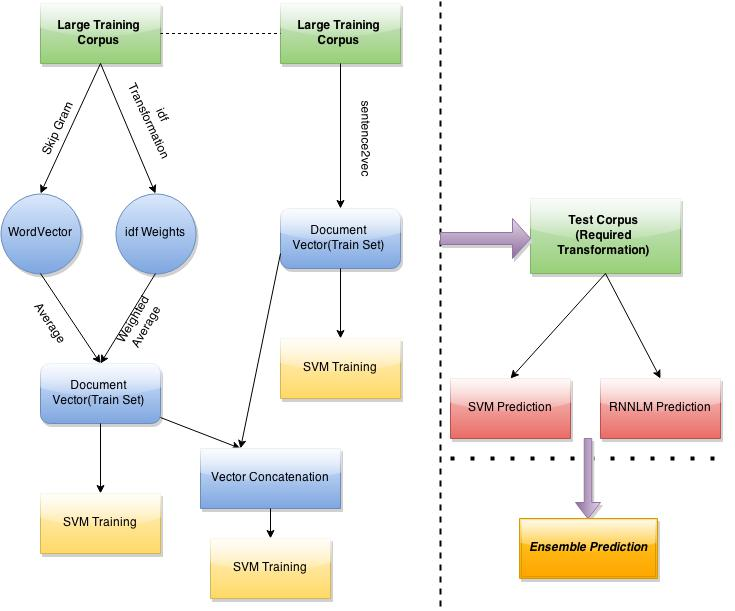
\includegraphics[width=160mm, height=180mm]{flow_chart.eps}
\caption{Work Flow Summary. \label{fig:flow_chart}}
\end{figure}


\section{Tools/Libraries}
\begin{itemize}
	\item Eclipse: An Integrated Development Environment helped speed up the process of coding and its subsequent debugging.
	\item Python: Being a very common and widely used programming language, loads of  documentation and third party libraries are available.
	\item Scikit: Open source library built on NumPy, SciPy and matplotlib which contains simple and efficient tools for data mining and data analysis.
	\item Gensim: It is an open-source vector space modeling and topic modeling toolkit, implemented in the Python programming language, using NumPy, SciPy and optionally Cython for performance. It is specifically intended for handling large text collections, using efficient online algorithms.
\end{itemize}
